% Author: Urs Zellweger (urs@zellweger.li)

\documentclass[11pt]{article}

	\usepackage{tikz}
	\usepackage{pgf}
	\usepackage{pgffor}
        \usepgfmodule{shapes}
        \usepgfmodule{plot}
        \usetikzlibrary{decorations}
        \usetikzlibrary{arrows}
    	\usetikzlibrary{snakes}

\newcommand{\physicalpendulum}{
        \pgfpathmoveto{\pgfpoint{0cm}{2cm}}
        \pgfpathcurveto{\pgfpoint{.2cm}{2cm}}{\pgfpoint{.2cm}{2cm}}{\pgfpoint{1cm}{1cm}}
        \pgfpathcurveto{\pgfpoint{1.75cm}{0cm}}{\pgfpoint{1.8cm}{0cm}}{\pgfpoint{2cm}{-2cm}}
        \pgfpathcurveto{\pgfpoint{2.2cm}{-4cm}}{\pgfpoint{2.3cm}{-4.2cm}}{\pgfpoint{2.5cm}{-5cm}}
        \pgfpathcurveto{\pgfpoint{2.7cm}{-5.8cm}}{\pgfpoint{3cm}{-6cm}}{\pgfpoint{3cm}{-7cm}}
        \pgfpathcurveto{\pgfpoint{3cm}{-8cm}}{\pgfpoint{2.25cm}{-8.75cm}}{\pgfpoint{2cm}{-9cm}}
        \pgfpathcurveto{\pgfpoint{1.75cm}{-9.25cm}}{\pgfpoint{1cm}{-10cm}}{\pgfpoint{0cm}{-10cm}}
        \pgfpathcurveto{\pgfpoint{-2cm}{-10cm}}{\pgfpoint{-3cm}{-8cm}}{\pgfpoint{-3cm}{-7cm}}
        \pgfpathcurveto{\pgfpoint{-3cm}{-3cm}}{\pgfpoint{-1cm}{-2cm}}{\pgfpoint{-1cm}{-1cm}}
        \pgfpathcurveto{\pgfpoint{-1cm}{0cm}}{\pgfpoint{-.5cm}{2cm}}{\pgfpoint{0cm}{2cm}}
        \pgfusepath{fill,stroke}
}

\begin{document}
    \begin{center}
        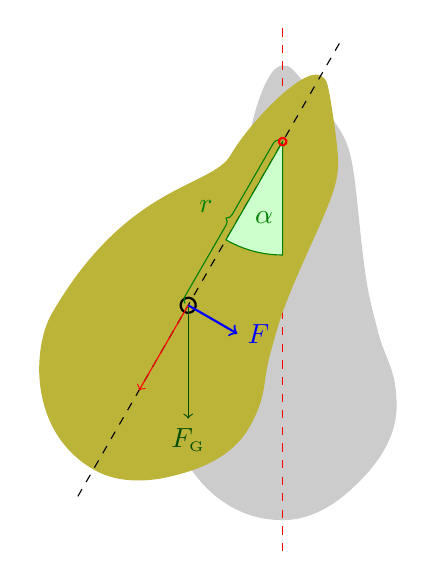
\begin{tikzpicture}[scale=.48]

            \color{black!20!white}
            \physicalpendulum

            \draw[color=red, dashed] (0,3)--(0,-11);

            \color{yellow!70!black}
            \pgftransformrotate{-30}
            \physicalpendulum


            \draw[color=black, dashed] (0,3)--(0,-11);
            \pgftransformrotate{30}
            \filldraw[fill=green!20,draw=green!50!black] (0,0) -- (0,-3) arc (-90:-120:3) -- cycle;
            \node[color=green!50!black] at (-.49,-2) {$\alpha$};
            \pgftransformrotate{-30}
            \draw[color=black, thick] (0,-5) circle (.2cm);
            \pgftransformrotate{30}
            \draw[->, color=green!30!black] (-2.5,-4.33)--(-2.5,-7.33) node[below] {$F_{\mbox{\tiny G}}$};
            \pgftransformrotate{-30}
            \draw[->, color=blue, thick] (0,-5)--(1.5,-5) node[right] {$F$};
            \draw[->, color=red] (0,-5)--(0,-7.6);
            \draw[snake=brace, color=green!50!black] (-.1,-5)--(-.1,0);
            \node[color=green!50!black] at (-.9,-2.5) {$r$};
            \draw[color=red, thick] (0,0) circle (.1cm);
        \end{tikzpicture}
    \end{center}
\end{document}
